\subsubsection{802.11}
% 
When wireless networks first came around, it was expected that the radio medium will only be another physical layer, such as cables. However, it did not take long to see that due to significant differences of radio communication, more detailed, radio-suited standard needs to be developed. In 1991 work has begun in preparation of standard that is today known as \emph{802.11} \cite{Hiertz2010TheUniverse}. The scope of this standard is \textquote[\cite{2016IEEEAccess.}]{\emph{to define one medium access control (MAC) and several physical layer specifications for wireless connectivity for fixed, portable, and moving stations within a local area.}}\par
One of the most well-known implementations of 802.11 is Wi-Fi. Naturally, it is not the only one and over the years, several amendments have been accepted to initial standard, to accommodate various needs. As Bilgin\&Gungor \cite{Bilgin2013PerformanceAreas} suggest, amendment 802.11b may be used in vehicular environment. Furthermore (and more importantly), amendment 802.11p has been published in 2010. This amendment is designed for the use in transportation, where communication window between two entities may only exist for very limited amount of time and thus some authentication procedures need to be omitted. We will discuss both amendments in following sections.
% 
% 
% 
\subsubsection{802.11b}
% 
The 802.11b uses the 2.4GHz unlicensed spectrum and provided increased maximum data rate of 11 Mb/s. It  modulates the data with spread spectrum modulation technique \emph{Direct-sequence spread spectrum} (DSSS). The spread spectrum modulation modifies the signal in a way, that broader spectrum is used than necessarily needed before modulation. Since the signal is spread over more frequencies, it is less vulnerable to interference \cite{MaximIntegratedProductsInc.2013AnMaxim}.
Similarly to the original standard, 802.11b uses the \emph{Distributed coordination function} (DCF) as the Medium access control (MAC) \cite{Hiertz2010TheUniverse}. DCF is a protocol that utilises \emph{Carrier-sense multiple access with collision avoidance} (CSMA/CA) together with binary exponential back-off algorithm. The CSMA/CA listens for broadcast on a channel and if there is none (of the channel is free) only then it starts broadcasting. The operation of CSMA/CA can be seen in detail in figure \ref{fig:csma-ca}.
% 
\begin{figure}
    \centering
    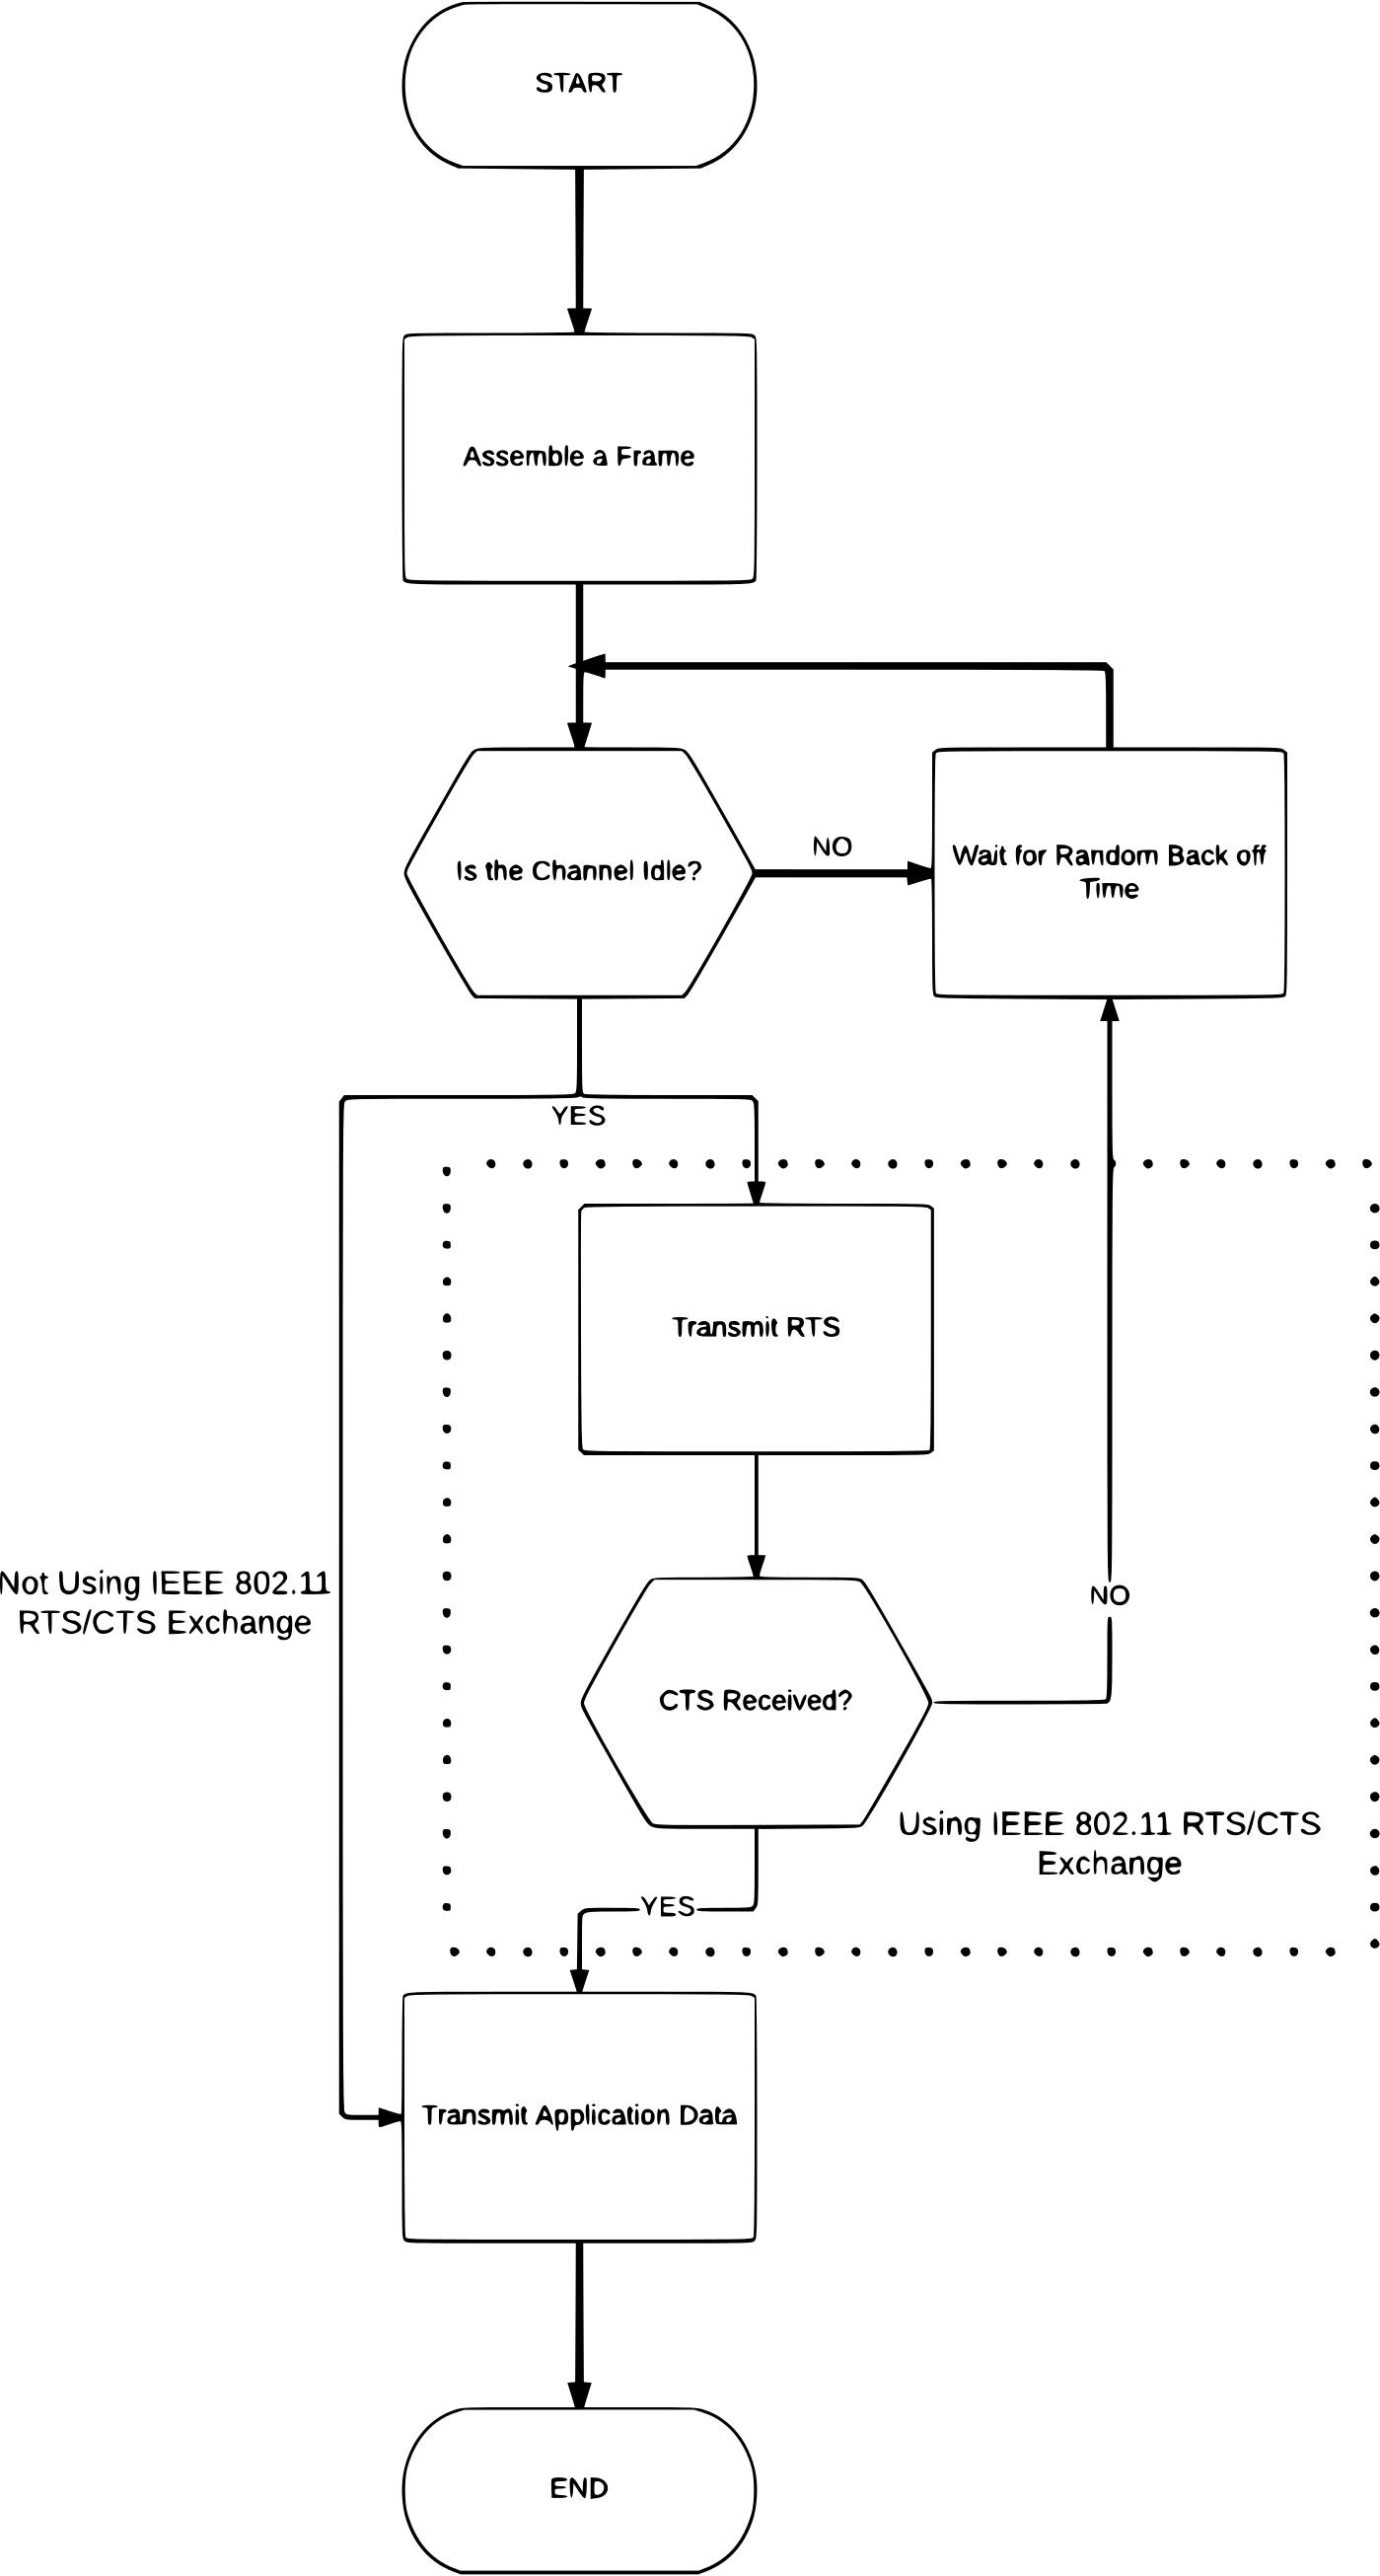
\includegraphics[height=.95\textheight]{csma-ca}
    \caption{Flowchart showing the operation of CSMA/CA. The dotted square shows RTS/CTS protocol, implementation of which is voluntary. RTS/CTS is part of 802.11 standard, but is not a part of 802.11b amendment. Source: \url{https://commons.wikimedia.org/wiki/File:Csma_ca.svg}}
    \label{fig:csma-ca}
\end{figure}
% 
\par // More info will follow here about how 802.11b is used in vehicular environment. I will investigate \cite{Bilgin2013PerformanceAreas}.